% !TeX program = lualatex
\documentclass[aspectratio=169]{../gpresentation}

%%% Checks whether a string is not given/empty/blank or not.
% Ex.: \NewDocumentCommand{\test}{O{}}{\IfEmptyTF{#1}{true}{false}}
% \text -> true
% \test[] -> true
% \test[   ] -> true
% \test[a] -> false
\ExplSyntaxOn
\cs_set_eq:NN\IfEmptyT\tl_if_blank:nT
\cs_set_eq:NN\IfEmptyF\tl_if_blank:nF
\cs_set_eq:NN\IfEmptyTF\tl_if_blank:nTF
\ExplSyntaxOff
\RequirePackage{marvosym}

\graphicspath{{img/}}

% This is a highly special setting, so it is set here.
\setbeamersize{description width of={Phase \phaseiii}}

\tikzset{
	legend/.style = {font=\boldmath, align=left},
	every path/.style = {line width=.57mm, line cap=round},
}

\subject{Seminar Approximation Algorithms}
\title[Approximating Nash Social Welfare under Submodular Valuations through (Un)Matchings]{Approximating Nash Social Welfare under Submodular Valuations \\ through (Un)Matchings}
\subtitle{Based on a paper of the same title by J. Garg, P\!. Kulkarni, and R. Kulkarni}
\author[Zeno Adrian Weil]{\texorpdfstring{Ƶ}{Z}eno Adrian \texorpdfstring{\Lss05{W\kern-1.25pt}}{W}eil}
\supervisor{Supervised by Dr Giovanna Varricchio}
\date[]{\today}
\institute[]{Algorithms and Complexity (Prof. Dr Martin Hoefer)}

\begin{document}
	\begin{frame}[plain, noframenumbering]
		\titlepage
	\end{frame}

	\begin{frame}{What is the issue?}{Introduction}
	\adjustfortopblock
	\begin{block}{}
		We need to distribute goods amongst recipients \emph{fast}, \emph{efficient} and \emph{fairly}.
	\end{block}

	Where is this encountered?
	\begin{itemize}
		\item
		industrial procurement

		\item
		cloud services

		\item
		satellites

		\item
		water withdrawal
	\end{itemize}

	\begin{center}
		\includegraphics[height=2cm]{img/industrialprocurement}
		\hfil
		\includegraphics[height=2cm]{img/cloudservices}
		\hfil
		
\includegraphics[height=2cm]{img/satellites}
		\hfil
		\includegraphics[height=2cm]{img/water}
	\end{center}
\end{frame}

	\begin{frame}{Table of Contents}
		\tableofcontents%[pausesections]
	\end{frame}

	\section{Preliminaries}

\subsection{Allocations}
\begin{frame}{Allocations}
	Setting:
	\adjustfortopitem
	\begin{itemize}
		\item
		recipients: set \(\agents\) of \(n\) agents

		\item
		goods: set \(\goods\) of \(m\) items
		\begin{itemize}
			\item
			unsharable

			\item
			indivisible
		\end{itemize}
	\end{itemize}
	\beamerimage at ( 8cm, 1.25cm) {\includegraphics[height=2cm]{img/nosatellites}};
	\beamerimage at (10cm, 1.25cm) {
\includegraphics[height=2cm]{img/nowater}};
	\vspace{-3ex}
	\begin{definition}[1]
		An \emph{allocation} is a tuple
		\(\alloc[][] = (\alloc)_{i \in \agents}\)
		of bundles \(\alloc \subset \goods\) such that each item is element of precisely one bundle.

		Item \(j\) is \emph{assigned} to agent \(i\) if \(j \in \alloc\).
	\end{definition}

	But how to measure its efficiency and fairness?
\end{frame}





\subsection{Valuation Functions}
\begin{frame}{Valuation Functions}{}
	Requirements:
	\adjustfortopitem
	\begin{itemize}
		\item
		monotonically non-decreasing: \(\valuations[\genericset[1]] \le \valuations[\genericset[2]]\) \quad \(\forall \genericset[1] \subset \genericset[2] \subset \goods\)

		\item
		normalised: \(\valuations[\emptyset] = 0\)

		\item
		non-negative: \(\valuations[\genericset] \ge 0\) \quad \(\forall \genericset \subset \goods\)
	\end{itemize}

	Types:
	\adjustfortopitem
	\begin{itemize}
		\item
		additive: \(\valuations[\genericset] \coloneq \sum_{\genericitem \in \genericset} \valuations[ \hairspace \genericitem ]\) \quad \(\forall \genericset \subset \goods\)

		\item
		submodular: \(\valuations[\genericset[1] \given \genericset[2]] \coloneq \valuations[\genericset[1] \cup \genericset[2]] - \valuations[\genericset[2]]\) \quad \(\forall \genericset[1], \genericset[2] \subset \goods\) with \(\genericset[1], \genericset[2]\) disjoint
		\begin{itemize}
			\item
			more general

			\item
			diminishing returns
		\end{itemize}
	\end{itemize}

	\begin{center}
		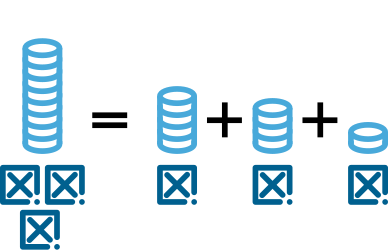
\includegraphics[height=2cm]{img/additive}
		\hfil
		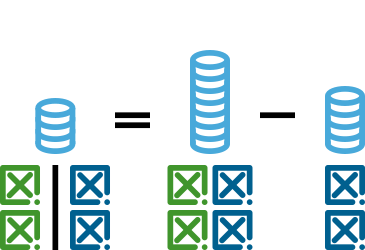
\includegraphics[height=2cm]{img/submodular}
		\hfil
		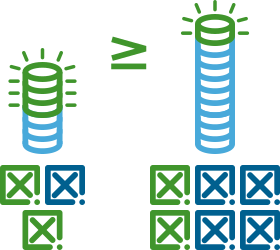
\includegraphics[height=2cm]{img/diminishingreturns}
	\end{center}
\end{frame}





\subsection{Maximum Nash Social Welfare Problem}
\begin{frame}{Asymmetric Maximum Nash Social Welfare Problem}
	\adjustfortopblock
	\begin{problem}[2]
		\begin{equation*}
			\alloc*[][] \overset{!}{=} \smashoperator{\argmax_{\alloc[][] \in \allallocs{\scriptstyle\agents\kern1pt}{\goods}}} \braces{ \NSW(\alloc[][]) }
			\quad\text{with~}
			\NSW(\alloc[][]) \coloneq \paren[\Big]{ \smashoperator{\prod_{i \in \agents}} \valuations[\alloc]^{\,\textstyle\weight} }{}^{\textstyle 1 / \sum_{i \in \agents} \weight}
		\end{equation*}
		\adjustfortopitem
		\begin{itemize}
			\item
			\(\allallocs{\agents\kern1pt}{\goods}\): all possible allocations

			\item
			\(\weight\): agent weight
		\end{itemize}
	\end{problem}
	The NSW strikes a middle ground between efficiency and fairness!
	\begin{alertblock}{}
		Is there a polynomial-time algorithm with an approximation factor \dots
		\begin{itemize}
			\item
			\dots{} dependent on \(n\)?

			\item
			\dots{} independent from \(m\)?
		\end{itemize}
		\beamerimage at (13cm, 1.15cm) {
\includegraphics[height=2cm]{img/nvsm}};
		\vspace{-0.75ex}
	\end{alertblock}
\end{frame}

	\section{RepReMatch}
\label{sec:reprematch}

\begin{algorithm*}[!b]
	\KwIn{%
		set \(\agents\) of \(n\) agents with weights \(\weight\) for all agents \(i \in \agents\),
		set \(\goods\) of indivisible \(m\) items,
		submodular valuations \(\valuations \colon \powerset[\goods] \to \realposzero\) where \(\valuations[\genericset]\) is the valuation of agent \(i \in \agents\) for each set \(\genericset \subset \goods\) of items
	}
	\KwOut{%
		\(\frac{1}{2n(\log_2 n + 3)}\)-approximation \(\alloc[\phaseiii][] = (\alloc[\phaseiii][1], \dots, \alloc[\phaseiii][n])\) of an optimal allocation
	}
	\phaseisep
	\(\alloc[\phasei] \gets \emptyset\)\;
	\(\goodsrem \gets \goods\)\;
	\For{\(t \gets 1, \dots, \ceil{\log_2 n}+1\)}{
		\If{\(\goodsrem \neq \emptyset\)}{
			\(\weights \gets \{\,  \weight \cdot \log\paren[\big]{ \valuations[j] } \given[\bigm] i \in \agents, j \in \goodsrem \,\}\)   \tct*{valuation of single item}
			\(\bipartitegraph \gets (\agents, \goodsrem, \weights)\)\;
			\(\matching \gets \maxweightmatching(\bipartitegraph)\)\;
			\(\alloc[\phasei] \gets \alloc[\phasei] \cup \{j\} \quad \forall(i, j) \in \matching\)\;
			\(\goodsrem \gets \goodsrem \setminus \{\, j \given (i, j) \in \matching \,\}\)\;
		}
	}
	\phaseiisep
	\(\alloc[\phaseii] \gets \emptyset \quad\forall i \in \agents\)   \tct*{put allocation \(\alloc[\phasei][]\) away and start a new one}
	\While{\(\goodsrem \neq \emptyset\)}{
		\(\weights \gets \{\,  \weight \cdot \log\paren[\big]{ \valuations[ \alloc[\phaseii] \cup \{j\} ] } \given[\bigm] i \in \agents, j \in \goodsrem \,\}\)   \tct*{val. of item \& cur. bundle}
		\(\bipartitegraph \gets (\agents, \goodsrem, \weights)\)\;
		\(\matching \gets \maxweightmatching(\bipartitegraph)\)\;
		\(\alloc[\phaseii] \gets \alloc[\phaseii] \cup \{j\} \quad \forall(i, j) \in \matching\)\;
		\(\goodsrem \gets \goodsrem \setminus \{\, j \given (i, j) \in \matching \,\}\)\;
	}
	\phaseiiisep
	\(\goodsrem \gets \mathop{\bigcup\hspace{-1pt}_{i \in \agents}} \alloc[\phasei]\)  \tct*{release items assigned in phase~\phasei} \label{ln:goodsrem}
	\(\weights \gets \{\,  \weight \cdot \log\paren[\big]{ \valuations[ \alloc[\phaseii] \cup \{j\} ] } \given[\bigm] i \in \agents, j \in \goodsrem \,\}\)   \tct*{val. of item \& cur. bundle}
	\(\bipartitegraph \gets (\agents, \goodsrem, \weights)\)  \label{ln:bipartitegraph}\;
	\(\matching \gets \maxweightmatching(\bipartitegraph)\)\;
	\(\alloc[\phaseiii] \gets \alloc[\phaseii] \cup \{j\} \quad\forall(i, j) \in \matching\)\;
	\(\goodsrem \gets \goodsrem \setminus \{\, j \given (i, j) \in \matching \,\}\)\;
	\(\alloc[\phaseiii][] \gets \arballoc( \agents, \goodsrem, \alloc[\phaseiii][], (\valuations)_{i \in \agents} )\)\;
	\Return{\(\alloc[\phaseiii][]\)}
	\caption{%
		\RepReMatch{} for the Asymmetric Submodular \NSW{} problem
	}
	\label{alg:reprematch}
\end{algorithm*}

The algorithm \SMatch{} estimates the valuation of the lowest-value items by determining the set of highest-value items and then valuing the remaining items.
Unfortunately, this approach does not work for general submodular valuations because taking the set of highest-value items away does not necessarily leave a set of lowest-value items.
In fact, it can be shown \cite{submodular_low_value} that determining the set of lowest-value items is approximable only within a factor of \(\bigomega(\sqrt{m / \ln m})\).

For this reason, the algorithm \RepReMatch, described in \cref{alg:reprematch}, relies on an approach with three phases, achieving an approximation factor of \(2n(\log_2 n + 3)\) (cf.\@ \cref{th:reprematch}).
In phase~\phasei, a sufficiently big set of high-value items is determined through repeated matchings.
This phase serves merley to determine this set, so items are assigned temporarily only.
The edge weights reflect this by taking the valuations of just single items into account.

In phase~\phaseii, the remaining items are assigned normally through repeated matchings.
Consequently, each edge weight is updated in each round to be the weighted logarithm of the valuation of both the respective item and the items assigned so far.

In phase~\phaseiii, the high-value items assigned in phase \phasei{} are released.
With the knowledge of items assigned in phase~\phaseii, one maximum weight matching is calculated, and the matched items are assigned accordingly.
Again each edge weight is the weighted logarithm of the valuation of both the respective item and the respective agent's bundle from phase \phaseii.
The remaining released items are assigned arbitrarily.

We start by analysing phase~\phaseii{} as it is the first phase with definitive assignments.
To this end, we introduce two types of item sets.
Note that we use the term \emph{round} to refer to the iterations of the loops in the phases~\phasei{} and~\phaseii.
For ease of notation, we refer to the moment before the first iteration in phase~\phaseii{} as round 0.
\begin{definition}
	Let \(\alloc*\) be an optimal allocation of some agent \(i \in \agents\).
	For any round \(r \ge 1\) in phase~\phaseii, the set \(\lostset{r} \subset \alloc*\) of \emph{lost} items is the set of all items \(j \in \alloc*\) assigned to other agents \(i' \neq i\) in that round.
\end{definition}
\begin{definition}
	Let \(\alloc*\) be an optimal allocation of some agent \(i \in \agents\) and \(\alloc[\phaseii] = \{ \asgd{1}, \dots, \asgd{\alloclen[\phaseii]} \}\) be her bundle in phase \phaseii.
	The set \(\attopt{r}\) of \emph{optimal and attainable} items is defined as \(\attopt{0} \coloneq \alloc* \setminus \mathop{\bigcup\hspace{-1pt}_{i' \in \agents}} \alloc[\phasei][i']\) in round \(0\) and as \(\attopt{r} \coloneq \attopt{r-1} \setminus ( \lostset{r} \cup \{\asgd{r-1}\}\) in round \(r \in [1, \alloclen[\phaseii]]\).
\end{definition}
We denote their sizes by \(\lostsetlen{r}\ \coloneq \abs{\lostset{r}}\) and \(\attoptlen{r} \coloneq \abs{\attopt{r}}\), respectively.\todo[info]{\(\mathbfit{i}\): Would it be \enquote{dirty} to include notation in the definitions?}
First, we give a lower bound on the valuations of optimal and attainable items.
\begin{lemma}
	\label{lem:induction}
	For each agent \(i \in \agents\) and her bundle \(\alloc[\phaseii] = \{ \asgd{1}, \dots, \asgd{\alloclen[\phaseii]} \}\), it holds in all rounds \(r = 2, \dots, \alloclen[\phaseii]\) of phase \phaseii{} that
	\begin{equation*}
		\valuations[ \attopt{r} \given \asgd{1}, \dots, \asgd{r-1} ] \geq \valuations[\attopt{1}] - \lostsetlen{2} \cdot \valuations[\asgd{1}] - \smashoperator{\sum_{r'=2}^{r-1}} \lostsetlen{r'} \cdot \valuations[ \asgd{r'} \given \asgd{1}, \dots, \asgd{r'-1} ] - \valuations[\asgd{1}, \dots, \asgd{r-1}].
	\end{equation*}
\end{lemma}
\begin{proof}
	We prove the lemma by induction on the number \(r\) of rounds.
	In the beginning of the base case \(r=2\), agent \(i\) has already been assigned item \(\asgd{1}\).
	For each of the optimal and attainable items~\(j \in \attopt{1}\) in round \(1\), the marginal valuation \(\valuations[j \given \emptyset]\) over the empty set was at most \(\valuations[\asgd{1} \given \emptyset]\), as otherwise item~\(\asgd{1}\) would not have been assigned first.
	The marginal valuation \(\valuations[j \given \asgd{1}]\) over \(\{\asgd{1}\}\) is upper-bounded by \(\valuations[\asgd{1} \given \emptyset]\), too, due to the submodularity of valuations.
	During round \(2\), a further \(\lostsetlen{2}\) of these items \(j\) are assigned to other agents, and item \(\asgd{2}\) is assigned to agent \(i\).
	We can bound the marginal valuation of the remaining optimal and attainable items in round \(2\) in the following way:
	\begin{caseintext}{1}{\(\asgd{1} \in \attopt{1}\)}
		It holds \(\valuations[ \attopt{2} \given \asgd{1} ] = \valuations[ \attopt{2} \cup \{\asgd{1}\} ] - \valuations[\asgd{1}] = \valuations[\attopt{1} \setminus \lostset{2}] -  \valuations[\asgd{1}]\).
	\end{caseintext}
	\begin{caseintext}{2}{\(\asgd{1} \notin \attopt{1}\)}
		Due to the monotonicity of valuations, it holds \(\valuations[ \attopt{2} \cup \{\asgd{1}\} ] \geq \valuations[ \attopt{2} ]\) and, therefore, \(\valuations[ \attopt{2} \given \asgd{1} ] \geq \valuations[ \attopt{2} ] - \valuations[\asgd{1}] = \valuations[\attopt{1} \setminus \lostset{2}] -  \valuations[\asgd{1}]\).
	\end{caseintext}
	\noindent
	In both cases, the base case is proven because
	\begin{align}
		\valuations[ \attopt{2} \given \asgd{1} ]
		&\geq \valuations[\attopt{1} \setminus \lostset{2}] -  \valuations[\asgd{1}] \\
		&\geq \valuations[ \attopt{1} ] - \valuations[\lostset{2}] - \valuations[\asgd{1}] \\
		&\geq \valuations[ \attopt{1} ] - \lostsetlen{2} \valuations[\asgd{1}] - \valuations[\asgd{1}],
	\end{align}
	where the second inequality can be shown inductively with the definition of submodularity\todo{Do that or, alternatively, find a paper showing the other def.}, and the third inequality is due all \(\lostsetlen{2}\) items \(j\) in set \(\lostset{2}\) not being assigned in round \(1\) although attainable, implying \(\valuations[j] \leq \valuations[\asgd{1}]\).

	For the induction hypothesis, we assume that the lemma holds true for all rounds up to some~\(r\).
	In the induction step \(r \to r+1\), we differentiate the same two cases again:
	\begin{caseintext}{1}{\(\asgd{r} \in \attopt{r}\)}
		Again we exploit the submodularity of valuations \todo{ditto} to obtain a lower bound on the marginal valuation of \(\attopt{r+1}\).
		\begin{align}
			\valuations[ \attopt{r+1} \given \asgd{1}, \dots, \asgd{r} ]
			&= \valuations[ \attopt{r+1} \cup \{\asgd{r}\} \given \asgd{1}, \dots, \asgd{r-1} ] - \valuations[ \asgd{r} \given \asgd{1}, \dots, \asgd{r-1} ] \\
			&= \valuations[ \attopt{r} \setminus \lostset{r+1} \given \asgd{1}, \dots, \asgd{r-1} ] - \valuations[ \asgd{r} \given \asgd{1}, \dots, \asgd{r-1} ] \\
			&\geq \begin{multlined}[t]
				\valuations[ \attopt{r} \given \asgd{1}, \dots, \asgd{r-1} ] - \valuations[ \asgd{r} \given \asgd{1}, \dots, \asgd{r-1} ] \\
				- \valuations[ \lostset{r+1} \given \asgd{1}, \dots, \asgd{r-1} ]
			\end{multlined}
		\end{align}
	\end{caseintext}
	\begin{caseintext}{2}{\(\asgd{r} \notin \attopt{r}\)}
		At first, we use the monotonicity of valuations to get the inequality
		\begin{align}
			\valuations[ \attopt{r} \given \asgd{1}, \dots, \asgd{r} ]
			&= \valuations[ \attopt{r} \cup \{ \asgd{1}, \dots, \asgd{r} \} ] - \valuations[\asgd{1}, \dots, \asgd{r}] \\
			&\geq \valuations[ \attopt{r} \cup \{ \asgd{1}, \dots, \asgd{r-1} \} ] - \valuations[\asgd{1}, \dots, \asgd{r}] \\
			&= \begin{multlined}[t]
				\paren[\big]{ \valuations[ \attopt{r} \cup \{ \asgd{1}, \dots, \asgd{r-1} \} ] - \valuations[\asgd{1}, \dots, \asgd{r-1}] } \\
				- \paren[\big]{ \valuations[\asgd{1}, \dots, \asgd{r}] - \valuations[\asgd{1}, \dots, \asgd{r-1}] }
			\end{multlined} \\
			&= \valuations[ \attopt{r} \given \asgd{1}, \dots, \asgd{r-1} ] - \valuations[ \asgd{r} \given \asgd{1}, \dots, \asgd{r-1} ].
		\end{align}
		Together with the submodularity of valuation, we obtain the same lower bound again:
		\begin{align}
			\valuations[ \attopt{r+1} \given \asgd{1}, \dots, \asgd{r} ]
			&= \valuations[ \attopt{r} \setminus \lostset{r+1} \given \asgd{1}, \dots, \asgd{r} ] \\
			&\geq \valuations[ \attopt{r} \given \asgd{1}, \dots, \asgd{r} ] - \valuations[ \lostset{r+1} \given \asgd{1}, \dots, \asgd{r} ] \\
			&\geq \valuations[ \attopt{r} \given \asgd{1}, \dots, \asgd{r} ] - \valuations[ \lostset{r+1} \given \asgd{1}, \dots, \asgd{r-1} ] \\
			&\geq \begin{multlined}[t]
				\valuations[ \attopt{r} \given \asgd{1}, \dots, \asgd{r-1} ] - \valuations[ \asgd{r} \given \asgd{1}, \dots, \asgd{r-1} ] \\
				- \valuations[ \lostset{r+1} \given \asgd{1}, \dots, \asgd{r-1} ]
			\end{multlined}
		\end{align}
	\end{caseintext}
	In both cases, we can replace \(\valuations[ \attopt{r} \given \asgd{1}, \dots, \asgd{r-1} ]\) by the induction hypothesis and \(\valuations[ \lostset{r+1} \given \asgd{1}, \dots, \asgd{r-1} ]\) by \(\lostsetlen{r+1} \cdot \valuations[ \asgd{r} \given \asgd{1}, \dots, \asgd{r-1} ]\) to prove the lemma.
	For a detailed calculation we refer to \citeauthor{APNSWuSVþUM}~\cite[14]{APNSWuSVþUM}.
	\todo{include if space enough}
\end{proof}

The lemma can be used to find a lower bound on the marginal valuation of the items assigned in each round \(r\).
\begin{corollary}
	\label{cor:lower_bound_single_item}
	From \cref{lem:induction} follows
	\begin{equation*}
		\valuations[ \asgd{r} \given \asgd{1}, \dots, \asgd{r-1} ] \geq \begin{multlined}[t]
			\paren[\Big]{ \valuations[\attopt{1}] - \lostsetlen{2} \cdot \valuations[\asgd{1}] - \smashoperator{\sum_{r'=2}^{r-1}} \lostsetlen{r'+1} \cdot \valuations[ \asgd{r'} \given \asgd{1}, \dots, \asgd{r'-1} ] \\
				- \valuations[\asgd{1}, \dots, \asgd{r-1}] } \Bigm/ \attoptlen{r}.
		\end{multlined}
	\end{equation*}
\end{corollary}
\begin{proof}
%	There are \(\attoptlen{0}\) optimal and attainable items in \(\attopt{0}\) at the start of phase~\phaseii.
%	Of those, \(\lostsetlen{l}\) many are assigned to other agents in each round \(l \leq r\), and also some items \(\asgd{l}\) assigned to agent \(i\) may be optimal, whence an upper bound of \(\attoptlen{0} - \sum_{l=1}^{r} \lostsetlen{l}\) on the number \(\attoptlen{r}\) of items in the set \(\attopt{r}\).\todo{Possibly this whole estimation can be omitted as we ditch it in the following lemma.}

	The valuations are monotonic, \ie, \(\valuations[\genericset[1]] \leq \valuations[\genericset[2]]\) for all item sets \(\genericset[1] \subset \genericset[2] \subset \goods\).\todo{change proof when intro is finished}
	Induction shows that there must be an item \(j \in \attopt{r}\) with a marginal valuation of at least \(\valuations[ \attopt{r} \given \asgd{1}, \dots, \asgd{r-1} ] / \attoptlen{r}\).
	As item \(\asgd{r}\) was the one to be assigned, the marginal valuation of it cannot be smaller.
	Using \cref{lem:induction} for the value of \(\valuations[ \attopt{r} \given \asgd{1}, \dots, \asgd{r-1} ]\) proves the corollary.
\end{proof}

This, finally, enables us to give a lower bound on the valuation of the whole bundle assigned in phase~\phaseii.
\begin{lemma}
	\label{lem:lower_bound_all_items}
	For each agent \(i \in \agents\) and her bundle \(\alloc[\phaseii] = \{\asgd{1}, \dots, \asgd{\alloclen[\phaseii]}\}\), it holds
	\begin{equation*}
		\valuations[\asgd{1}, \dots, \asgd{\alloclen[\phaseii]}] \geq \valuations[\attopt{1}] / n.
	\end{equation*}
\end{lemma}
\begin{proof}
	In each round \(r = 1, \dots, \alloclen[\phaseii]\), \(\lostsetlen{r}\) optimal and attainable items of agent \(i\) are assigned to other agents.
	As there are \(n\) agents in total, \(n-1\) is an upper bound on \(\lostsetlen{r}\).
	Furthermore, after \(\alloclen[\phaseii]\) rounds, the number \(\attoptlen{\alloclen[\phaseii]}\) of optimal and attainable items is at most \(n-1 \leq n\) elsewise agent \(i\) would have been assigned yet another item.
	Together with \cref{cor:lower_bound_single_item}, this proves the lemma:
	\begin{align}
		\valuations[\asgd{1}, \dots, \asgd{\alloclen[\phaseii]}]
		&= \valuations[ \asgd{\alloclen[\phaseii]} \given \asgd{1}, \dots, \asgd{\alloclen[\phaseii]} ] + \valuations[\asgd{1}, \dots, \asgd{\alloclen[\phaseii] - 1}] \\
		&\geq \begin{multlined}[t]
			\paren[\Big]{ \valuations[\attopt{1}] - \lostsetlen{2} \cdot \valuations[\asgd{1}]
				- \smashoperator{\sum_{r'=2}^{\alloclen[\phaseii]-1 \mathstrut}} \lostsetlen{r'+1} \cdot \valuations[ \asgd{r'} \given \asgd{1}, \dots, \asgd{r'-1} ] \\
				- \valuations[\asgd{1}, \dots, \asgd{\alloclen[\phaseii]-1}] } \Big/ \attoptlen{r} + \valuations[\asgd{1}, \dots, \asgd{\alloclen[\phaseii] - 1}]  % \Big/ has better spacing than \Bigm/.
		\end{multlined} \\
		&\geq \begin{multlined}[t]
			\paren[\Big]{ \valuations[\attopt{1}] - (n-1) \valuations[\asgd{1}]
				- \smashoperator{\sum_{r'=2}^{\alloclen[\phaseii]-1 \mathstrut}} (n-1) \valuations[ \asgd{r'} \given \asgd{1}, \dots, \asgd{r'-1} ] \\
				- \valuations[\asgd{1}, \dots, \asgd{\alloclen[\phaseii]-1}] } \Big/ n + \valuations[\asgd{1}, \dots, \asgd{\alloclen[\phaseii] - 1}]
		\end{multlined} \\
		&\geq \begin{multlined}[t]
			\paren[\big]{ \valuations[\attopt{1}] - (n-1) \valuations[\asgd{1}, \dots, \asgd{\alloclen[\phaseii]-1}] - \valuations[\asgd{1}, \dots, \asgd{\alloclen[\phaseii]-1}] } \big/ n \\
			+ \valuations[\asgd{1}, \dots, \asgd{\alloclen[\phaseii] - 1}]
		\end{multlined} \\
		&= \valuations[\attopt{1}] / n
	\end{align}
\end{proof}

After having obtained a lower bound on the valuation of items assigned in phase~\phaseii, we need a lower bound for phase~\phaseiii{} as well.
Therefor we introduce a third type of item set.
\begin{definition}
	Let \(\alloc* = \{ \asgd*{1}, \dots, \asgd{\alloclen*}\}\) be an optimal allocation of some agent \(i \in \agents\).
	The set \(\overlygoodset\) of \emph{overly good} items is defined as \(\overlygoodset \coloneq \{\, j \in \goods \given \valuations[j] \geq \valuations[\asgd*{1}] \,\}\).
\end{definition}

\begin{lemma}
	\label{lem:overly_good_matching}
	In phase~\phaseiii, there exists a matching such that each agent \(i \in \agents\) is matched to one of her overly good items in the set \(\mathop{\bigcup\hspace{-1pt}_{i' \in \agents}} \alloc[\phasei][i']\) of released items.
\end{lemma}
\begin{proof}
	If all items were matched in phase~\phasei, \ie, \(\mathop{\bigcup\hspace{-1pt}_{i' \in \agents}} \alloc[\phasei][i'] = \goods\), then all optimal items are released in phase~\phaseiii{} and each agent can be matched to one;
	the lemma is proven immediately.
	If not, imagine for some~\(t\) that only the items assigned in the first~\(t\) rounds of phase~\phasei{} were released.
%	Denote the set of released items by \(\goodsreleased{t}\).
	Now choose some matching \(\matching[t]\) with the following properties:
	\begin{enumerate}[topsep=0.1em, itemsep=0.1em, parsep=0pt]
		\item
		\label[property]{enum:matching:agent}
		If for an agent \(i\) all overly good items were amongst the released items,
%		\ie, \(\overlygoodset \subset \goodsreleased{t}\),
		she gets matched with an overly good item \(j \in \overlygoodset\).

		\item
		\label[property]{enum:matching:max}
		The number of agents matched with one of their overly good items is maximal amongst all matchings fulfilling \cref{enum:matching:agent}.
	\end{enumerate}
	\Cref{enum:matching:agent} is always satisfiable as each set \(\overlygoodset\) is the only one to contain the item \(\asgd*{1}\), which can be matched with agent \(i\).
	\Cref{enum:matching:max} leads to all agents being matched with an overly good item for \(t = \ceil{\log_2 n}+1\), \ie{} the number of rounds in phase~\phasei, whence the lemma follows.
	To prove this, we denote by \(\unluckyagents{t}\) the set of agents who are \emph{not} matched with one of their overly good items, and show by induction on \(t\) that it holds \(\abs{\unluckyagents{t}} \leq n/2^t\).

	In the base case \(t=1\), none of the items are assigned initially.
	Denote by \(\unluckyagentsalgo{1}\) the number of agents who were not assigned an overly good item in the first round of phase~\phasei.
	If \(\unluckyagentsalgo{1} \leq n/2\), then a matching \(\matching[1]\) obviously exists and the base case is immediately proven.
	Otherwise, all items from at least \(\unluckyagentsalgo{1}\) many sets \(\overlygoodset\) got assigned to someone.
	Again:
	Each set \(\overlygoodset\) is the only one containing the item \(\asgd*{1}\), so the union of these sets contains at least~\(\unluckyagentsalgo{1}\) items which can be matched with at least \(\unluckyagentsalgo{1}\) agents upon release.
	This then leaves at most~\(n-\alpha < n/2\) agents not matched with an overly good item.

	For the induction hypothesis, we assume that the statement holds true for all rounds up to some \(t\).
	In the induction step \(t \to t+1\), by \cref{enum:matching:agent}, there is at least one unassigned item in each set \(\overlygoodset[i']\) for all agents \(i' \in \unluckyagents{t}\) at the start of round \(t+1\).
	Analogously to the base case, for at least half of those agents \(i'\) these unassigned items will be assigned to them or someone else and it can be argued accordingly.
	By the induction hypothesis, it holds \(\abs{\unluckyagents{t+1}} \leq \abs{\unluckyagents{t}}/2 \leq (n/2^t)/2 = n/2^{t+1}\).
\end{proof}

This allows us to calculate an approximation factor for \RepReMatch{} by comparing its output with an optimal allocation \(\alloc*[][]\).
\begin{theorem}
	\label{th:reprematch}
	\RepReMatch{} has an approximation factor of \(2n (\log_2 n + 3)\).
\end{theorem}
\begin{proof}
	By \cref{lem:overly_good_matching}, we can assign each agent \(i\) an overly good item \(\overlygooditem \in \overlygoodset\) in the beginning of phase~\phaseiii.
	\RepReMatch{} maximises the logarithmic Nash social welfare, so
	\begin{equation}
		\label{eq:reprematch_approx_factor_lower_bound}
		\log \NSW(\alloc[\phaseiii][])
		\geq \frac{1}{\sum_{i \in \agents} \weight} \cdot \sum_{i \in \agents} \weight \log \valuations[\overlygooditem, \asgd{1}, \dots, \asgd{\alloclen[\phaseii]}]
	\end{equation}
	is a lower bound on the logarithmic \NSW{} after the first matching in phase~\phaseiii, whereby \(\alloc[\phaseii] = \{ \asgd{1}, \dots, \allowbreak \asgd{\alloclen[\phaseii]} \}\) is the bundle of agent \(i\) from phase~\phaseii.

	Item \(\overlygooditem\) was released in phase~\phaseiii, which means it was assigned in phase~\phasei, implying \(\overlygooditem \in \alloc* \setminus \attopt{0}\) and, subsequently, \(\overlygooditem \in (\alloc* \setminus \attopt{0}) \cup \lostset{1}\).
	Phase~\phasei{} runs for at most \(\ceil{\log_2 n}+1\)\todo[info]{\(\mathbfit{i}\): Error in paper‽ see also \cref{lem:overly_good_matching}} rounds, and at most \(n\) items are assigned in each iteration.
	Therefore, at most \(n (\log_2 n + 2)\) optimal items are assigned in that phase, \ie, \(\abs{ \alloc* \setminus \attopt{0} } \leq n (\log_2 n + 2)\).
	Furthermore, it holds \(n \geq \lostsetlen{1} = \abs{\lostset{1}}\) as in \cref{lem:lower_bound_all_items}.
	Together with the monotonicity of valuations, this yields
	\begin{equation}
		\label{eq:overly_good_item_lower_bound}
		\valuations[ \overlygooditem, \asgd{1}, \dots, \asgd{\alloclen[\phaseii]} ]
		\geq \valuations[\overlygooditem]
		\geq \frac{\valuations[ (\alloc* \setminus \attopt{0}) \cup \lostset{1} ][\big]}{n(\log_2 n + 3)}
	\end{equation}
	as lower bound on the valuations of bundles.
	Moreover, \cref{lem:lower_bound_later_items} and the monotonicity of valuations yield
	\begin{equation}
		\label{eq:assigned_items_lower_bound}
		\valuations[ \overlygooditem, \asgd{1}, \dots, \asgd{\alloclen[\phaseii]} ]
		\geq \valuations[ \asgd{1}, \dots, \asgd{\alloclen[\phaseii]} ]
		\geq \frac{\valuations[\attopt{1}]}{n}
		\geq \frac{\valuations[\attopt{1}]}{n(\log_2 n + 3)}
		= \frac{\valuations[ \attopt{0} \setminus \lostset{1} ]}{n(\log_2 n + 3)}
	\end{equation}
	as yet another lower bound.
	The mean of \crefrange{eq:overly_good_item_lower_bound}{eq:assigned_items_lower_bound} and the monotonicity of valuations give the concise lower bound
	\begin{align}
		\valuations[ \overlygooditem, \asgd{1}, \dots, \asgd{\alloclen[\phaseii]} ]
		&\geq \frac{1}{2} \paren*{ \frac{\valuations[ (\alloc* \setminus \attopt{0}) \cup \lostset{1} ][\big]}{n(\log_2 n + 3)} + \frac{\valuations[ \attopt{0} \setminus \lostset{1} ][\big]}{n(\log_2 n + 3)} } \\
		&\geq \frac{1}{2} \cdot \frac{ \valuations[ \paren{(\alloc* \setminus \attopt{0}) \cup \lostset{1}} \cup \paren{\attopt{0} \setminus \lostset{1}} ][\big] }{n(\log_2 n + 3)} \\
		&= \frac{ \valuations[\alloc*] }{2n(\log_2 n + 3)}.
	\end{align}
	We can insert this lower bound into \cref{eq:reprematch_approx_factor_lower_bound} and prove the theorem thereby:
	\begin{equation}
		\log \NSW(\alloc[\phaseiii][])
		\geq \frac{1}{\sum_{i \in \agents} \weight} \cdot \sum_{i \in \agents} \weight \log \paren[\bigg]{ \frac{ \valuations[\alloc*] }{2n(\log_2 n + 3)} }
		= \log \paren[\bigg]{ \frac{\NSW(\alloc*[][])}{2n(\log_2 n + 3)} }
	\end{equation}
\end{proof}

	\section{conclusion}
\label{sec:conclusion}

\begin{itemize}
	\item
	Of course a short rehearsal of the results for the now knowledgeable reader.

	\item
	An outlook would be nice to have.
	Its content would mostly depend on what recent research has not yet answered.
	\begin{itemize}
		\item
		conclusion of \cite{min_envy_and_max_avg_nsw_in_the_alloc_of_indiv_goods}

		\item
		cf. \cite{min_envy_and_max_avg_nsw_in_the_alloc_of_indiv_goods}: do not only approximate efficiency but also fairness

		\item
		https://www.semanticscholar.org/reader/bef4514574543720bc45ea235df4c4556e97efe0

		\item
		B. R. Chaudhury, Y. K. Cheung, J. Garg, N. Garg, M. Hoefer, and K. Mehlhorn. Fair division
		of indivisible goods for a class of concave valuations. J. Artif. Intell. Res., 74:111–142, 2022
	\end{itemize}
\end{itemize}

\lipsum[1-5]
\end{document}